\chapter{Using Dartel \label{Chap:dartelguide}}
\minitoc

\vskip 1.5cm

Dartel\footnote{Dartel stands for ``Diffeomorphic Anatomical Registration Through Exponentiated Lie algebra''.
It may not use a true Lie Algebra, but the acronym is a nice one.} is a suite of tools for achieving more accurate inter-subject registration of brain images.
It consists of several thousand lines of code. Because it would be a shame if this effort was wasted, this guide was written to help encourage its widespread use.
Experience at the FIL would suggest that it offers very definite improvements for VBM studies -- both in terms of localisation\footnote{Less smoothing is needed, and there are fewer problems relating to how to interpret the differences.} and increased sensitivity\footnote{More sensitivity could mean that fewer subjects are needed, which should save shed-loads of time and money.}.



\section{Using Dartel for VBM \label{Sec:dartel_vbm}}
The following procedures could be specified one at a time, but it is easier to use the batching system.
The sequence of jobs (use the \emph{Batch} button to start the batch manager) would be:
\begin{itemize}
\item{{\bf Module List}
  \begin{itemize}
  \item{{\bf SPM$\rightarrow$Spatial$\rightarrow$Segment}: To generate the roughly (via a rigid-body) aligned grey and white matter images of the subjects.}
  \item{{\bf SPM$\rightarrow$Tools$\rightarrow$Dartel Tools$\rightarrow$Run Dartel (create Template)}: Determine the nonlinear deformations for warping all the grey and white matter images so that they match each other.}
  \item{{\bf SPM$\rightarrow$Tools$\rightarrow$Dartel Tools$\rightarrow$Normalise to MNI Space}: Actually generate the smoothed ``modulated'' warped grey and white matter images.}
  \end{itemize}
}
\end{itemize}

Further details of the steps are described next.


\subsection{Using Spatial$\rightarrow$Segment}
\emph{Note: This subsection will be elaborated on later.}

The first step is to classify T1-weighted scans\footnote{Other types of scan may also work, but this would need some empirical exploration.} of a number of subjects into different tissue types via the Segmentation routine in SPM \cite{ashburner05}, which can be found under SPM$\rightarrow$Spatial$\rightarrow$Segment.
With this option, the ``imported'' tissue class images (usually rc1.nii and rc2.nii) would be generated directly.
It is also suggested that \emph{Native Space} versions of the tissues in which you are interested are also generated.
For VBM, these  are usually the c1*.nii files, as it is these images that will eventually be warped to MNI space.
Both the imported and native tissue class image sets can be specified via the Native Space options of the user interface.

Segmentation can require quite a lot of memory, so if you have large images (typically greater than about $256\times256\times150$) and trying to run it on a 32 bit computer or have relatively little memory installed, then it may throw up an out of memory error.
 
\subsection{Using Dartel Tools$\rightarrow$Run Dartel (create Template)}
The output of the previous step(s) are a series of rigidly aligned tissue class images (grey matter is typically encoded by rc1*.nii and white matter by rc2*.nii -- see Fig \ref{Fig:VBM}).
The headers of these files encode two affine transform matrices, so the Dartel tools are still able to relate their orientations to those of the original T1-weighted images.
The next step is to estimate the nonlinear deformations that best align them all together \cite{ashburner07}.
This is achieved by alternating between building a template, and registering the tissue class images with the template, and the whole procedure is very time consuming.
Specify \emph{SPM$\rightarrow$Tools$\rightarrow$Dartel Tools$\rightarrow$Run Dartel (create Template)}.
\begin{itemize}
\item{{\bf Run Dartel (create Template)}
  \begin{itemize}
  \item{{\bf Images}
    \begin{itemize}
    \item{{\bf Images}: Select all the rc1*.nii files generated by the import step.
    }
    \item{{\bf Images}: Select all the rc2*.nii files, in the same subject order as the rc1*.nii files. The first rc1*.nii is assumed to correspond with the first rc2*.nii, the second with the second, and so on.
    }
    \end{itemize}
  }
  \item{{\bf Settings}: Default settings generally work well, although you could try changing them to see what happens. A series of templates are generated called Template\_basename\_0.nii, Template\_basename\_1.nii etc.  If you run multiple Dartel sessions, then it may be a good idea to have a unique template basename for each. 
  }
  \end{itemize}
}
\end{itemize}
The procedure begins by computing an initial template from all the imported data.
If u\_rc1*.nii files exist for the images, then these are treated as starting estimates and used during the creation of the initial template.  If any u\_rc1*.nii files exist from previous attempts, then it is usually recommended that they are removed first (this sets all the starting estimates to zero).
Template generation incorporates a smoothing procedure \cite{john_averageshape}, which may take a while (several minutes).
Once the original template has been generated, the algorithm will perform the first iteration of the registration on each of the subjects in turn.
After the first round of registration, a new template is generated (incorporating the smoothing step), and the second round of registration begins.
Note that the earlier iterations usually run faster than the later ones, because fewer ``time-steps'' are used to generate the deformations.
The whole procedure takes (in the order of) about a week of processing time for 400 subjects.

\begin{figure}
\begin{center}
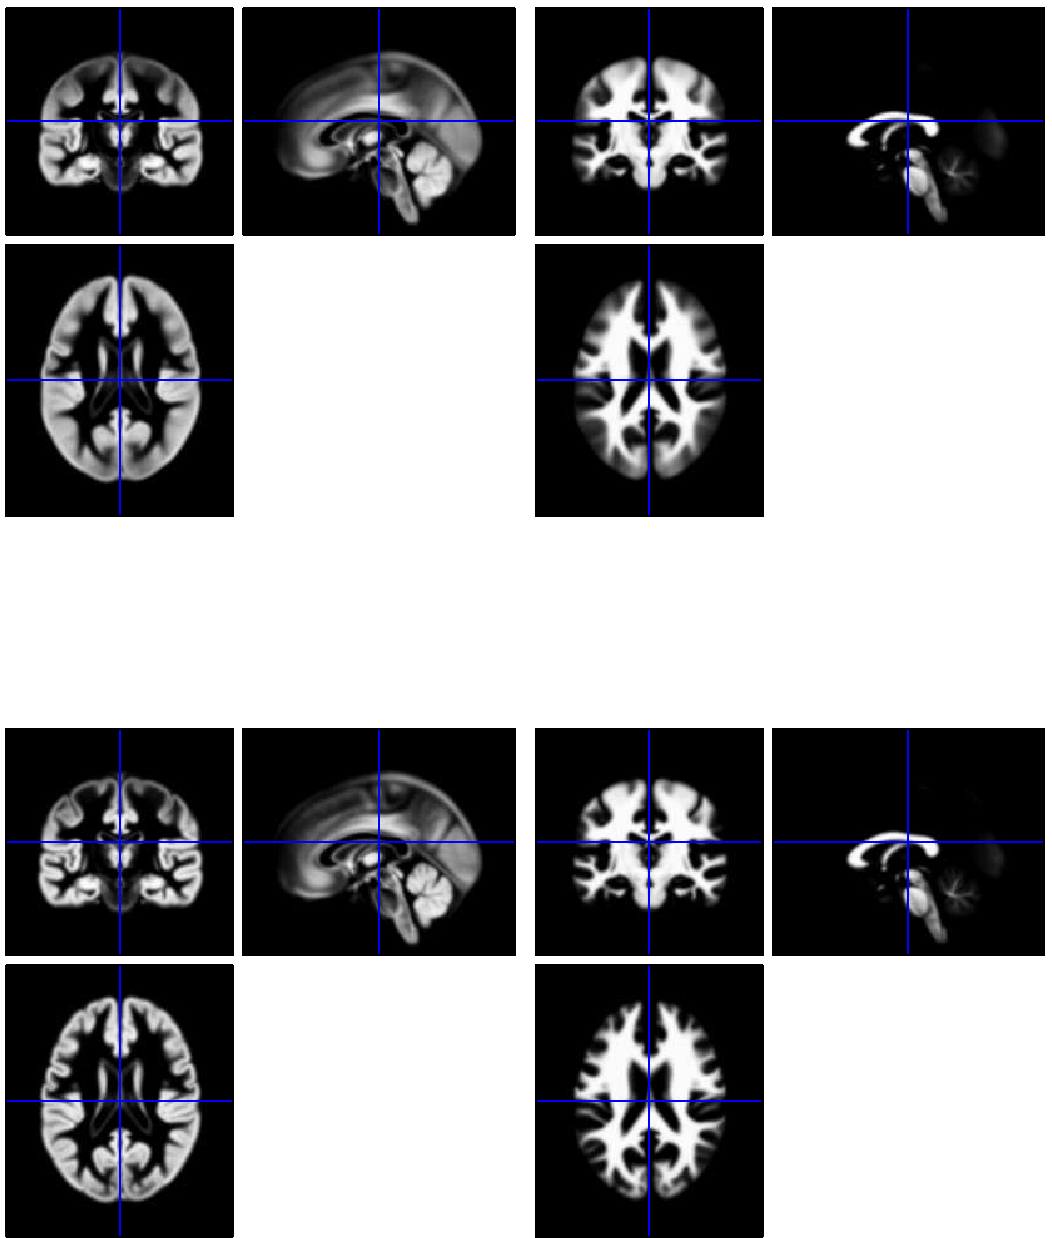
\epsfig{file=dartelguide/sharpening,width=140mm}
\end{center}
\caption{
Different stages of template generation.
Top row: an intermediate version of the template.
Bottom row: the final template data.
\label{Fig:sharpening}}
\end{figure}

The end result is a series of templates (see Fig \ref{Fig:sharpening}), and a series of u\_rc1*.nii files.
The first template is based on the average\footnote{They are actually more similar to weighted averages, where the weights are derived from the Jacobian determinants of the deformations. There is a further complication in that a smoothing procedure is built into the averaging.} of the original imported data, where as the last is the average of the Dartel registered data.
The u\_rc1*.nii files are flow fields that parameterise the deformations.
Note that all the output usually contains multiple volumes per file.
For the u\_rc1*.nii files, only the first volume is visible using the Display or Check Reg tools in SPM.
All volumes within the template images can be seen, but this requires the file selection to be changed to give the option of selecting more than just the first volume (in the file selector, the widget that says ``1'' should be changed to ``1:2'').

\subsection{Using Dartel Tools$\rightarrow$Normalise to MNI Space}
The next step is to create the Jacobian scaled (``modulated'') warped tissue class images, by selecting \emph{SPM$\rightarrow$Tools$\rightarrow$Dartel Tools$\rightarrow$Normalise to MNI Space}.
The option for spatially normalising to MNI space automatically incorporates an affine transform that maps from the population average (Dartel Template space) to MNI space, as well as incorporating a spatial smoothing step.
\begin{itemize}
\item{{\bf Normalise to MNI Space}
  \begin{itemize}
  \item{{\bf Dartel Template}: Specify the last of the series of templates that was created by \emph{Run Dartel (create Template)}.  This is usually called \emph{Template\_6.nii}.  Note that the order of the \emph{N} volumes in this template should match the order of the first \emph{N} volumes of the \emph{toolbox/Dartel/TPM.nii} file.}
  \item{{\bf Select according to} either \emph{Few Subjects} or \emph{Many Subjects}.  For VBM, the \emph{Many Subjects} option would be selected.
    \begin{itemize}
    \item{{\bf Flow Fields}: Specify the flow fields (u\_rc1*.nii) generated by the nonlinear registration.}
    \item{{\bf Images}: You may add several different sets of images.
      \begin{itemize}
      \item{{\bf Images}: Select the c1*.nii files for each subject, in the same order as the flow fields are selected.}
      \item{{\bf Images}: This is optional, but warped white matter images can also be generated by selecting the c2*.nii files.}
      \end{itemize}}
    \end{itemize}}
    \item{{\bf Voxel sizes}: Specify the desired voxel sizes for the spatially normalised images (NaN, NaN, NaN gives the same voxel sizes as the Dartel template).}
    \item{{\bf Bounding box}: Specify the desired bounding box for the spatially normalised images (NaN, NaN, NaN; NaN NaN NaN gives the same bounding box as the Dartel template).}
    \item{{\bf Preserve}: Here you have a choice of \emph{Preserve Concentrations} (ie not Jacobian scaled) or \emph{Preserve Amount} (Jacobian scaled).  The \emph{Preserve Amount} would be used for VBM, as it does something similar to Jacobian scaling (modulation).}
    \item{{\bf Gaussian FWHM}: Enter how much to blur the spatially normalised images, where the values denote the full width at half maximum of a Gaussian convolution kernel, in units of mm. Because the inter-subject registration should be more accurate than when done using other SPM tools, the FWHM can be smaller than would be otherwise used.  A value of around 8mm (ie $[8, 8, 8]$) should be about right for VBM studies, although some empirical exploration may be needed.  If there are fewer subjects in a study, then it may be advisable to smooth more.}
  \end{itemize}
}
\end{itemize}

The end result should be a bunch of smwc1*.nii files\footnote{The actual warping of the images is done slightly differently, with the aim that as much of the original signal is preserved as possible.  This essentially involves pushing each voxel from its position in the original image, into the appropriate location in the new image - keeping a count of the number of voxels pushed into each new position.  The procedure is to scan through the original image, and push each voxel in turn.  The alternative (older way) was to scan through the spatially normalised image, filling in values from the original image (pulling the values from the original).  The results of the pushing procedure are analogous to Jacobian scaled (``modulated'') data. A minor disadvantage of this approach is that it can introduce aliasing artifacts (think stripy shirt on TV screen) if the original image is at a similar - or lower - resolution to the warped version. Usually, these effects are masked by the smoothing.} (possibly with smwc2*.nii if white matter is also to be studied).

\begin{figure}
\begin{center}
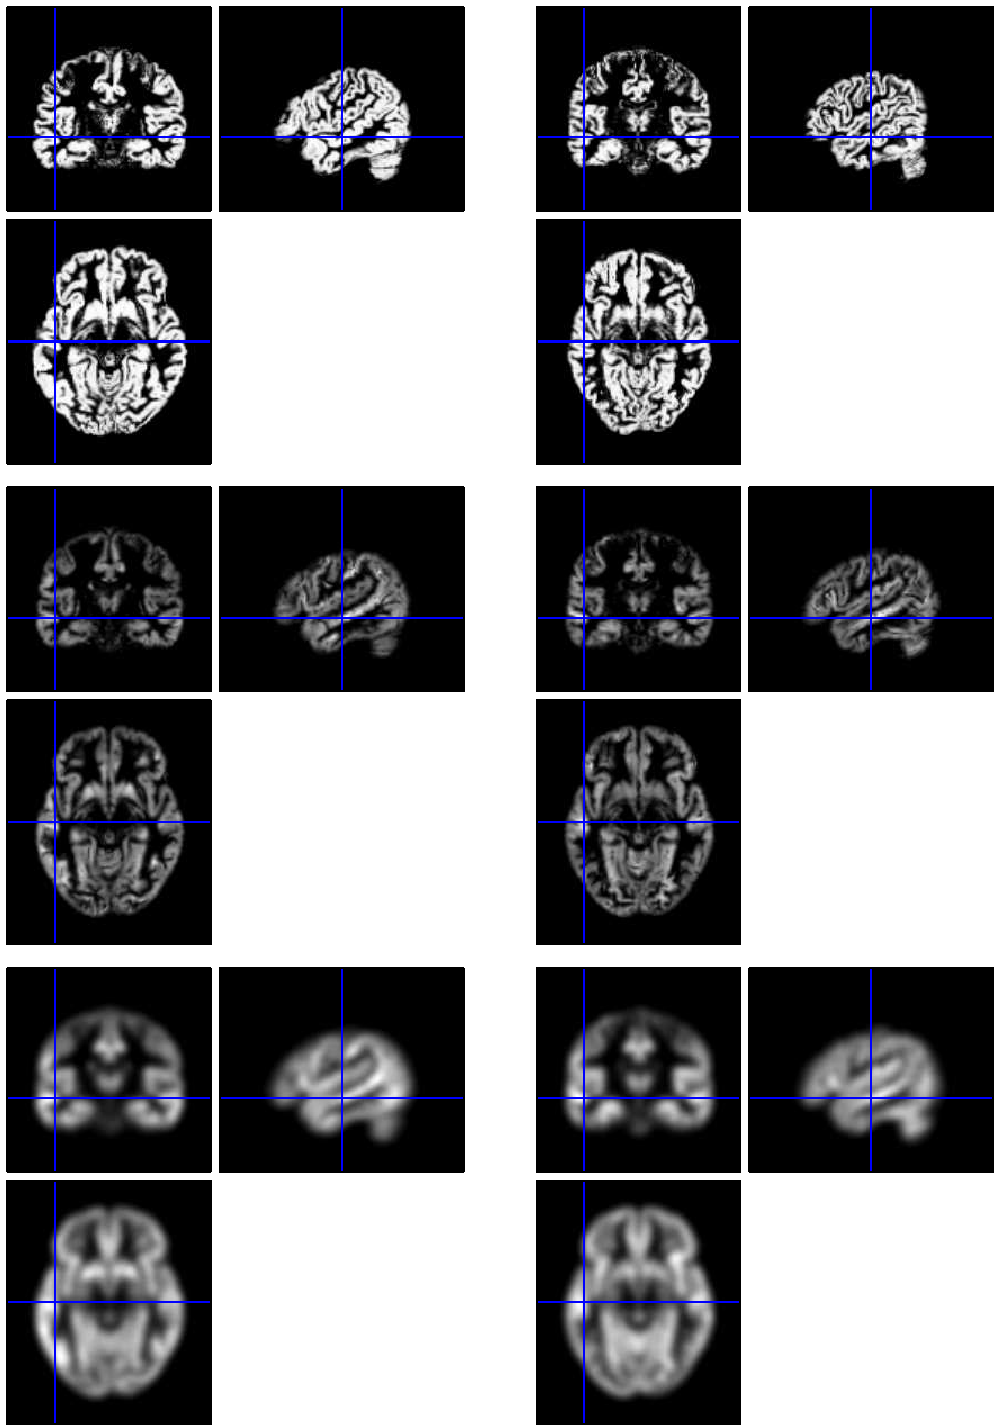
\epsfig{file=dartelguide/VBM,width=140mm}
\end{center}
\caption{
Pre-processing for VBM.
Top row: Imported grey matter (rc1A.nii and rc1B.nii).
Centre row: Warped with \emph{Preserve Amount} option and zero smoothing (``modulated'').
Bottom row: Warped with \emph{Preserve Amount} option smoothing of 8mm (smwc1A.nii and smwc1B.nii).
\label{Fig:VBM}}
\end{figure}

The final step is to perform the statistical analysis on the preprocessed data (smwc1*.nii files), which should be in MNI space.
The next section says a little about how data from a small number of subjects could be warped to MNI space.



\section{Spatially normalising functional data to MNI space}
Providing it is possible to achieve good alignment between functional data from a particular subject and an anatomical image of the same subject (distortions in the fMRI may prevent accurate alignment), then it may be possible to achieve more accurate spatial normalisation of the fMRI data using Dartel.
There are several advantages of having more accurate spatial normalisation, especially in terms of achieving more significant activations and better localisation.

The objectives of spatial normalisation are:
\begin{itemize}
\item{To transform scans of subjects into alignment with each other.
Dartel was developed to achieve better inter-subject alignment of data.
}
\item{To transform them to a standard anatomical space, so that activations can be reported within a standardised coordinate system.
Extra steps are needed to achieve this aim.
}
\end{itemize}

The option for spatially normalising to MNI space automatically incorporates an affine transform that maps from the population average (Dartel Template space) to MNI space.
This transform is estimated by minimising the KL divergence between the final template image generated by Dartel and tissue probability maps that are released as part of SPM's segmentation \cite{ashburner05}.  MNI space is defined according to affine matched images, so an affine transform of the Dartel template to MNI space would appear to be a reasonable strategy.

For GLM analyses, we usually do not wish to work with Jacobian scaled data.
For this reason, warping is now combined with smoothing, in a way that may be a bit more
sensible than simply warping, followed by smoothing.  The end result is
essentially the same as that obtained by doing the following with the old way of warping
\begin{itemize}
\item{Create spatially normalised and ``modulated'' (Jacobian scaled) functional data, and smooth.}
\item{Create spatially normalised maps of Jacobian determinants, and smooth by the same amount.}
\item{Divide one by the other, adding a small constant term to the denominator to prevent divisions by zero.}
\end{itemize}
This should mean that signal is averaged in such a way that as little as possible
is lost.  It also assumes that the procedure does not have any nasty side
effects for the GRF assumptions used for FWE corrections.

Prior to spatially normalising using Dartel, the data should be processed as following:
\begin{itemize}
\item{If possible, for each subject, use \emph{SPM$\rightarrow$Tools$\rightarrow$FieldMap} to derive a distortion field that can be used for correcting the fMRI data.
More accurate within-subject alignment between functional and anatomical scans should allow more of the benefits of Dartel for inter-subject registration to be achieved.}
\item{Use either \emph{SPM$\rightarrow$Spatial$\rightarrow$Realign$\rightarrow$Realign: Estimate Reslice} or \emph{SPM$\rightarrow$Spatial$\rightarrow$Realign Unwarp}.  If a field map is available, then use the \emph{Realign Unwarp} option.
The images need to have been realigned and resliced (or field-map distortion corrected) beforehand - otherwise things are not handled so well.  The first reason for this is that there are no options to use different methods of interpolation, so rigid-body transforms (as estimated by Realign but without having resliced the images) may not be well modelled.  Similarly, the spatial transforms do not incorporate any masking to reduce artifacts at the edge of the field of view.}
\item{For each subject, register the anatomical scan with the functional data (using \emph{SPM $\rightarrow$ Spatial $\rightarrow$ Coreg $\rightarrow$ Coreg: Estimate}).  No reslicing of the anatomical image is needed.
Use \emph{SPM$\rightarrow$Util$\rightarrow$Check Registration} to assess the accuracy of the alignment.
If this step is unsuccessful, then some pre-processing of the anatomical scan may be needed in order to skull-strip and bias correct it.
Skull stripping can be achieved by segmenting the anatomical scan, and masking a bias corrected version (which can be generated by the segmentation option) by the estimated GM, WM and CSF.  This masking can be done using \emph{SPM$\rightarrow$Util$\rightarrow$Image Calculator} (\emph{ImCalc} button), by selecting the bias corrected scan (m*.img), and the tissue class images (c1*.img, c2*.img and c3*.img) and evaluating ``i1.\*((i2+i3+i4)$>$0.5)''.
If segmentation is done before coregistration, then the functional data should be moved so that they align with the anatomical data.}
\item{Segment the anatomical data and generate ``imported'' grey and white matter images.}
\item{To actually estimate the warps, use \emph{SPM$\rightarrow$Tools$\rightarrow$Dartel Tools$\rightarrow$Run Dartel (create Templates)} in order to generate a series of templates and a flow field for each subject.}
\end{itemize}

In principle (for a random effects model), you could run the first level analysis using the native space data of each subject.
All you need are the contrast images, which can be warped and smoothed.
Alternatively, you could warp and smooth the reslices fMRI, and do the statistical analysis on the spatially normalised images.
Either way, you would select \emph{SPM$\rightarrow$Tools$\rightarrow$Dartel Tools$\rightarrow$Normalise to MNI Space}:
\begin{itemize}
\item{{\bf Normalise to MNI Space}
    \begin{itemize}
    \item{{\bf Dartel Template}: Template\_6.nii,1 is usually the grey matter component of the final template of the series.  An affine transform is determined using this image.}
    \item{{\bf Select according to} either \emph{Few Subjects} or \emph{Many Subjects}.  For fMRI analyses, the \emph{Few Subjects} option would be selected, which gives the option of selecting a flow field and list of images for each subject.
      \begin{itemize}
      \item{{\bf Subject}
        \begin{itemize}
        \item{{\bf Flow Field}: Specify the flow field (``u\_c1*.nii'') for this subject.}
        \item{{\bf Images}: Select the images for this subject that are to be transformed to MNI space.}
        \end{itemize}
      }
      \end{itemize}
    }
    \item{{\bf Voxel sizes}: Specify the desired voxel sizes for the spatially normalised images (NaN, NaN, NaN gives the same voxel sizes as the Dartel template).}
    \item{{\bf Bounding box}: Specify the desired bounding box for the spatially normalised images (NaN, NaN, NaN; NaN NaN NaN gives the same bounding box as the Dartel template).}
    \item{{\bf Preserve}: Here you have a choice of \emph{Preserve Concentrations} (ie not Jacobian scaled) or \emph{Preserve Amount} (Jacobian scaled).  The \emph{Preserve Concentrations} option would normally be used for fMRI data, whereas \emph{Preserve Amount} would be used for VBM.}
    \item{{\bf Gaussian FWHM}: Enter how much to blur the spatially normalised images, where the values denote the full width at half maximum of a Gaussian convolution kernel, in units of mm.}
    \end{itemize}
}
\end{itemize}

%An alternative approach is now presented, which does not attempt to make optimal use of the available signal.
%
%\subsection{An alternative approach for using Dartel to spatially normalise to MNI Space}
%During spatial normalisation of a brain image, some regions need to expanded and other regions need to contract in order to match the template.
%If some structure is excessively shrunk by Dartel (because it has the freedom to estimate quite large deformations), then this will lead to a systematic reduction in the amount of BOLD signal being detected from that brain region.
%For this reason, the normalise to MNI space option would generally be preferred when working with functional data that is to be smoothed.
%
%\subsubsection{Affine transform of Dartel template to MNI space}
%Dartel works with images that are of average size.
%When Dartel is used to generate an average shaped template (represented by a series of tissue probability maps) from a group of scans of various individuals, the result is of average size.
%Brains normalised to MNI space are slightly larger  than average.
%In order to spatially normalise to MNI space, the deformation that maps from MNI space to the space of the group average is required.
%Because the MNI space was derived by affine registration of a number of subjects to a common coordinate system, in most cases it should be possible to achieve a reasonable match of the template generated by Dartel using only an affine spatial normalisation.
%This can be achieved by matching the grey matter component of the template with a grey matter tissue probability map in MNI space.
%The spatial normalisation routine in SPM can be used to achieve this.

%\begin{itemize}
%\item{{\bf Normalise: Estimate}
%  \begin{itemize}
%  \item{{\bf Data}
%    \begin{itemize}
%    \item{{\bf Subject}
%      \begin{itemize}
%      \item{{\bf Source Image}: Template\_6.nii,1 is usually the grey matter component of the final template of the series.}
%      \item{{\bf Source Weighting Image}: $<$None$>$}
%      \end{itemize}
%    }
%    \end{itemize}
%  }
%  \item{{\bf Estimation Options}
%    \begin{itemize}
%    \item{{\bf Template Image}: Should be the apriori/grey.nii file distributed in SPM.}
%    \item{{\bf Template Weighting Image}: $<$None$>$}
%    \item{{\bf Source Image Smoothing}: 8mm (the same as the apriori/grey.nii file has been smoothed).}
%    \item{{\bf Template Image Smoothing}: 0mm (because the data in the apriori folder are already smoothed by 8mm.)}
%    \item{{\bf Affine Regularisation}: Usually, you would specify ``ICBM space template''.}
%    \item{{\bf Nonlinear Frequency Cutoff}: Set this to infinity (enter ``Inf'') for affine registration.}
%    \item{{\bf Nonlinear Iterations}: Setting this to zero will also result in affine-only spatial normalisation.}
%    \item{{\bf Nonlinear Regularisation}: Setting this to infinity is another way of doing affine-only spatial normalisation.}
%    \end{itemize}
%  }
%  \end{itemize}
%}
%\end{itemize}

%For some populations of subjects, an affine transform may not be adequate for achieving good registration of the average shape to MNI space.
%Nonlinear spatial normalisation may be more appropriate for these cases.
%As ever, determining which procedure is better would involve a degree of empirical exploration.
%
%\subsubsection{Combining deformations}
%Once you have the spatial transformation that maps from MNI space to the space of the Dartel template, it is possible to combine this with the DEFORMATIONS estimated by Dartel.
%Rather than warping the image data twice (introducing interpolation artifacts each time), the two spatial transforms can be combined by composing them together.
%The required deformation, for spatially normalising an individual to MNI space, is a mapping from MNI space to the individual image.
%This is because the spatially normalised images are generated by scanning through the (initially empty) voxels in the spatially normalised image, and figuring out which voxels in the original image to sample from (as opposed to scanning through the original image and putting the values into the right places in the spatially normalised version).
%
%The desired mapping is from MNI space to Dartel template to individual scan.
%If \emph{A} is the mapping from MNI to template, and \emph{B} is the mapping from template to individual, then this mapping is $B \circ A$, where ``$\circ$'' denotes the composition operation.
%Spatially normalising via the composed deformations can be achieved through the \emph{Deformations} utility. 
%
%\begin{itemize}
%\item {\bf Deformations}
%  \begin{itemize}
%  \item {\bf Composition}
%    \begin{itemize}
%    \item {\bf Dartel flow}
%      \begin{itemize}
%      \item {\bf Flow field}: Specify the u\_rc1*.nii flow field for that subject.
%      \item {\bf Forward/Backwards}: This should be set to ``Backward'' to indicate a mapping from template to individual.
%      \item {\bf Time Steps}: This is the number of time steps used by the final iterations of the Dartel registration (usually 64).
%      \item {\bf Dartel template}: leave this field empty.
%      \end{itemize}
%    \item {\bf Imported \_sn.mat}
%      \begin{itemize}
%      \item {\bf Parameter File}: Select the spatial normalisation parameters that would spatially normalise the Template\_6.nii file.
%      \item {\bf Voxel sizes}: These are set to ``NaN'' (not a number) by default, which would take the voxel sizes for the apriori/grey.nii file.  Alternatively, you could specify your favourite voxel sizes for spatially normalised images.
%      \item {\bf Bounding box}: Again, these are set to non-finite values by default, which results in the same bounding box as the apriori/grey.nii file.  To specify your favourite bounding box, enter $[x_{min}, y_{min}, z_{min}; x_{max}, y_{max}, z_{max}]$ (in units of mm, relative to the AC).
%      \end{itemize}
%    \end{itemize}
%  \item {\bf Output}
%    \begin{itemize}
%    \item {\bf Pullback}
%      \begin{itemize}
%      \item {\bf Apply to}: Specify the images for that subject that you would like spatially normalised.
%      \item {\bf Output destination}: Specify where you want to write the images.
%      \item {\bf Interpolation}: Specify the form of interpolation.
%      \item {\bf Mask images}: Say whether you want to mask the images (see the Chapter on Realignment for more information here).
%      \item {\bf Gaussian FWHM}: The images can be smoothed when they are written.  If you do not want this, then enter 0 0 0.
%      \end{itemize}
%    \end{itemize}
%  \end{itemize}
%\end{itemize}

%The above procedure would be repeated for each subject in the study.

\section{Warping Images to Existing Templates}
If templates have already been created using Dartel, then it is possible to align other images with such templates.
The images would first be imported in order to generate rc1*.nii and rc2*.nii files.
The procedure is relatively straight-forward, and requires the \emph{SPM$\rightarrow$Tools$\rightarrow$Dartel Tools$\rightarrow$Run Dartel (existing Template)} option to be specified.
Generally, the procedure would begin by registering with a smoother template, and end with a sharper one, with various intermediate templates between.
\begin{itemize}
\item{{\bf Run Dartel (existing Templates)}
  \begin{itemize}
  \item{{\bf Images}
    \begin{itemize}
    \item{{\bf Images}: Select the rc1*.nii files.}
    \item{{\bf Images}: Select the corresponding rc2*.nii files.}
    \end{itemize}
  }
  \item{{\bf Settings}: Most settings would be kept at the default values, except for the specification of the templates.
These are specified in within each of the \emph{Settings$\rightarrow$Outer Iterations$\rightarrow$Outer Iteration$\rightarrow$Template} fields.
If the templates are Template\_*.nii, then enter them in the order of Template\_1.nii, Template\_2.nii, ... Template\_6.nii.
  }
  \end{itemize}
}
\end{itemize}

Running this option is rather faster than \emph{Run Dartel (create Template)}, as templates are not created.
The output is in the form of a series of flow fields (u\_rc1*.nii).

\section{Warping one individual to match another}
Sometimes the aim is to deform an image of one subject to match the shape of another.
This can be achieved by running Dartel so that both images are matched with a common template, and composing the resulting spatial transformations.
This can be achieved by aligning them both with a pre-existing template, but it is also possible to use the \emph{Run Dartel (create Template)} option with the imported data of only two subjects.
Once the flow fields (u\_rc1*.nii files) have been estimated, then the resulting deformations can be composed using \emph{SPM$\rightarrow$Utils$\rightarrow$Deformations}.
If the objective is to warp A.nii to align with B.nii, then the procedure is set up by:
\begin{itemize}
\item {\bf Deformations}
  \begin{itemize}
  \item {\bf Composition}
    \begin{itemize}
    \item {\bf Dartel flow}
      \begin{itemize}
      \item {\bf Flow field}: Specify the u\_rc1A\_Template.nii flow field.
      \item {\bf Forward/Backwards}: Backward.
      \item {\bf Time Steps}: Usually 64.
      \item {\bf Dartel template}: leave this field empty.
      \end{itemize}
    \item {\bf Dartel flow}
      \begin{itemize}
      \item {\bf Flow Field}: Specify the u\_rc1B\_Template.nii flow field.
      \item {\bf Forward/Backwards}: Forward.
      \item {\bf Time Steps}: Usually 64.
      \item {\bf Dartel template}: leave this field empty.
      \end{itemize}
    \item {\bf Identity}
      \begin{itemize}
      \item {\bf Image to base Id on}: Specify B.nii in order to have the deformed image(s) written out at this resolution, and with the same orientations etc (ie so there is a voxel-for-voxel alignment, rather than having the images only aligned according to their ``voxel-to-world'' mappings).
      \end{itemize}
    \end{itemize}
  \item {\bf Output}
    \begin{itemize}
    \item {\bf Pullback}
      \begin{itemize}
      \item {\bf Apply to}: Specify A.nii, and any other images for that subject that you would like warped to match B.nii. Note that these other images must be in alignment according to \emph{Check Reg}.
      \item {\bf Output destination}: Specify where you want to write the images.
      \item {\bf Interpolation}: Specify the form of interpolation.
      \item {\bf Mask images}: Say whether you want to mask the images.
      \item {\bf Gaussian FWHM}: The images can be smoothed when they are written.  If you do not want this, then enter 0 0 0.
      \end{itemize}
    \end{itemize}
  \end{itemize}
\end{itemize}

Suppose the image of one subject has been manually labelled, then this option is useful for transferring the labels on to images of other subjects.

\begin{figure}
\begin{center}
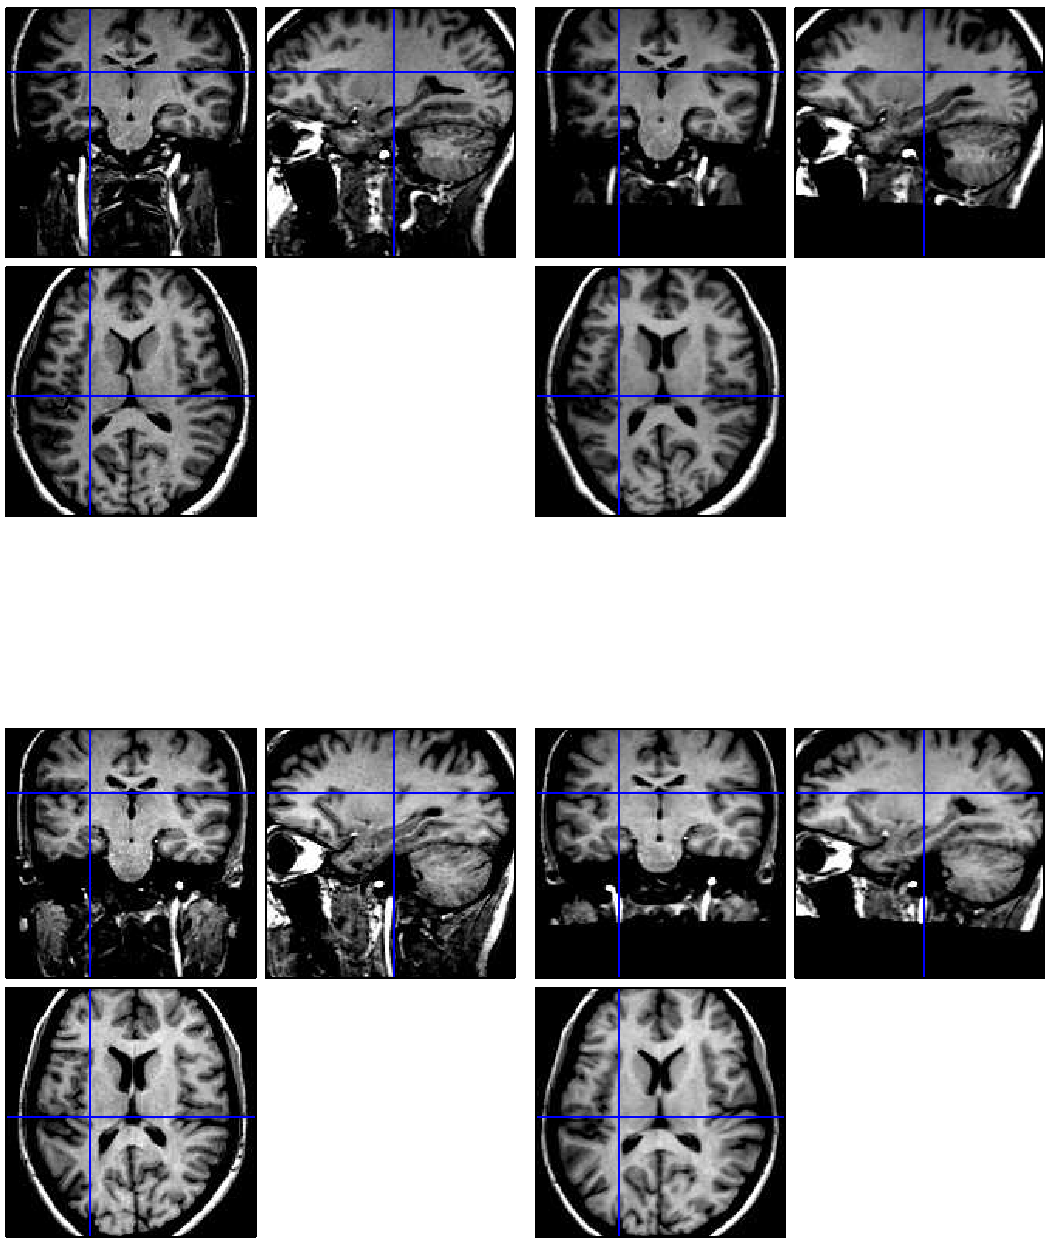
\epsfig{file=dartelguide/AtoB,width=140mm}
\end{center}
\caption{
Composition of deformations to warp one individual to match another.
Top-left: Original A.nii.
Top-right: A.nii warped to match B.nii.
Bottom-left: Original B.nii.
Bottom-right: B.nii warped to match A.nii.
\label{Fig:AtoB}}
\end{figure}


